\documentclass[border=12pt,11pt]{standalone}
\usepackage{tikz}
\usetikzlibrary{arrows.meta}

% ---- font size knobs ----
\newcommand{\vtxfont}{\normalsize}   % vertex names
\newcommand{\caplabel}{\small}       % capacity labels

\begin{document}
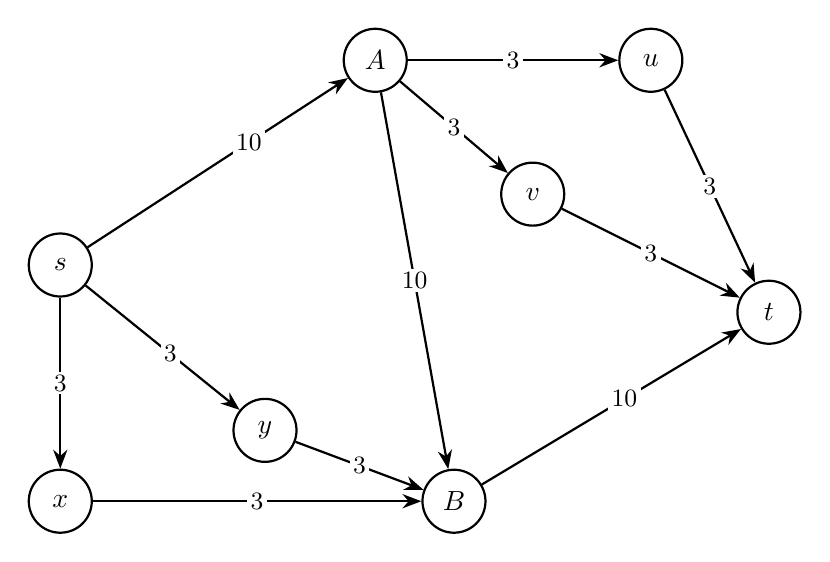
\begin{tikzpicture}[
  >={Stealth[length=2.4mm]},
  vtx/.style={circle,draw,thick,fill=white,minimum size=8mm,inner sep=0pt,
              font=\vtxfont},
  ed/.style={->,thick},
  lbl/.style={font=\caplabel,fill=white,inner sep=1.2pt}
]

% ---------- vertices ----------
\node[vtx] (S) at (0,0)      {$s$};
\node[vtx] (A) at (4,2.6)    {$A$};
\node[vtx] (U) at (7.5,2.6)  {$u$};
\node[vtx] (V) at (6,0.9)    {$v$};
\node[vtx] (T) at (9,-0.6)   {$t$};
\node[vtx] (X) at (0,-3)     {$x$};
\node[vtx] (Y) at (2.6,-2.1) {$y$};
\node[vtx] (B) at (5,-3)     {$B$};

% ---------- edges with capacities ----------
\draw[ed] (S) -- (A) node[lbl,pos=0.62] {$10$};
\draw[ed] (S) -- (X) node[lbl,pos=0.5]  {$3$};
\draw[ed] (S) -- (Y) node[lbl,pos=0.55] {$3$};
\draw[ed] (X) -- (B) node[lbl,pos=0.5]  {$3$};
\draw[ed] (Y) -- (B) node[lbl,pos=0.5]  {$3$};
\draw[ed] (A) -- (U) node[lbl,pos=0.5]  {$3$};
\draw[ed] (U) -- (T) node[lbl,pos=0.5]  {$3$};
\draw[ed] (A) -- (V) node[lbl,pos=0.5]  {$3$};
\draw[ed] (V) -- (T) node[lbl,pos=0.5]  {$3$};
\draw[ed] (A) -- (B) node[lbl,pos=0.5]  {$10$};
\draw[ed] (B) -- (T) node[lbl,pos=0.55] {$10$};

\end{tikzpicture}
\end{document}
